        \documentclass{standalone}
        \usepackage{tikz}
        \begin{document}
        \fontsize{16px}{16px}\selectfont
        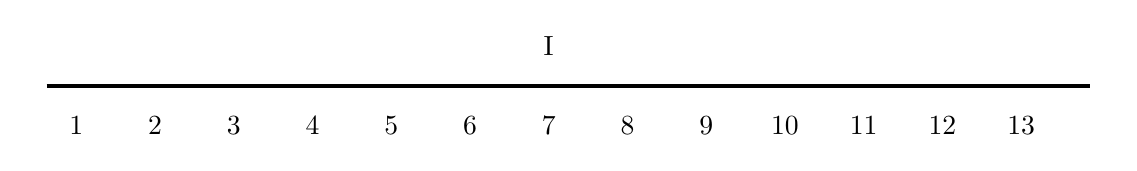
\begin{tikzpicture}

    \node at (-0.5,0.5) (nodeAA) {};
    \node at (0,0) (nodeA) {1};
    \node at (1,0) (nodeB) {2};
    \node at (2,0) (nodeC) {3};
    \node at (3,0) (nodeD) {4};
    \node at (4,0) (nodeE) {5};
    \node at (5,0) (nodeF) {6};
    \node at (6,0) (nodeG) {7};
    \node at (7,0) (nodeH) {8};
    \node at (8,0) (nodeI) {9};
    \node at (9,0) (nodeJ) {10};
    \node at (10,0) (nodeK) {11};
    \node at (11,0) (nodeL) {12};
    \node at (12,0) (nodeM) {13};
    \node at (13,0.5) (nodeMM) {};
    \node at (6,1) (nodemid) {I};
    \draw[ultra thick](nodeAA) -- (nodeMM);
        \end{tikzpicture}
        \end{document}
